\documentclass[]{article}
\usepackage[utf8]{inputenc}
%\usepackage[danish, english]{babel}
\usepackage[danish]{babel}
\usepackage{graphicx}
%\usepackage[intoc]{nomencl} % Nomenclature package
\usepackage[usenames]{xcolor}
\usepackage{times}
\usepackage{listings}
\usepackage{textcomp}
\usepackage{hyperref}
\usepackage{textpos}
\usepackage{pgfgantt}
\usepackage{lscape}
%\usepackage[showboxes]{textpos}
\usepackage{indentfirst}
\usepackage{tikz}
\usepackage{pgfplots}
\usepackage{ifthen}
\usepackage{float}
%\usepackage{mathtools}
\usepackage{pict2e}
%\usepackage{steinmetz}
\usepackage[export]{adjustbox}
\pgfplotsset{compat=1.13}
\usepackage{siunitx}
\usepackage{tabularx}
%
% adjustment to page format
\marginparwidth=0pt
\oddsidemargin=0pt
%\evensidemargin=0pt
\marginparsep=0pt
%\topmargin=-15 mm
\textwidth=168 mm
\textheight=230 mm
\parskip 0.27 em
\parindent=0pt
%\leftmargin=1cm

% Define DTU color
\definecolor{dtured}{RGB}{153,0,0}
\title{Projektplan}
\begin{document}
% formel header
\thispagestyle{empty}
\vspace*{-1.9cm}
\begin{textblock*}{18cm}[0,0](0cm,-2cm) %
  \noindent
  
\includegraphics[width=4.5cm,valign=t]{documentation/resources/tex_dtu_elektro_a.pdf}
  \hspace*{10.6cm}
  
\includegraphics[width=1.5cm,valign=t]{documentation/resources/tex_dtu_logo.pdf}
\end{textblock*}
\begin{textblock*}{19.0cm}(0cm,-2.5cm) %
\begin{center}
  {\color{dtured}\large31015 Fagprojekt}\\
  \normalsize
  s186083 Tjark Petersen\\
  s194006 Steffan Martin Kunoy\\
  s194027 Victor Alexander Hansen\\
\end{center}
\end{textblock*}
% rød streg
\vspace{1mm}
{\hspace*{-0.1cm}
\color{dtured}\noindent \rule{16.8cm}{5pt}}
 
\begin{table}[H]
     \centering
     \begin{tabularx}{\textwidth}{|X|X|X|}
     \hline
          DTU Elektro&Forår 2021 & Gruppe: 7, ID: MEK2 \\\hline
          Kursus 31015 & Titel & Gruppemedlemmer \\\hline
          Fagprojekt - Elektroteknologi & ROAST Telemetri & \begin{tabular}{l} s186083 Tjark Petersen\\s194006 Steffan Martin Kunoy\\s194027 Victor Alexander Hansen \end{tabular}\\\hline
          Dokument:& Projektformulering & 1 side\\\hline 
          Version/Status: & 1. udgave &\today\\\hline
     \end{tabularx}
 \end{table}
 
\section{Introduktion til emne/problemstilling}

Dette projekt vil omhandle et telemetri modul som skal indgå i DTU Roadrunners Solar Team (ROAST). I 2023 deltager ROAST i Bridgestone World Solar Challenge, som er et løb på over 3000 km tværs gennem Australien \cite{wsc}. Solbilen skal køre en distance på 3 x 1200km, hvor bilen ikke har mulighed for at oplade. Den primære energikilde for bilen under løbet er derfor solenergi.\\
I løbet vil solbilen være ledsaget af en følgebil, som skal overvåge solbilens driftstatus og sende kommandoer til solbilen. Dette er en yderst vigtig opgave, da bilerne skal køre tværs gennem Australien i offentlig trafik, hvor alt fra varme til dæktryk udfordrer solbilen. Følgebilen vil derfor have mulighed for at analysere og reagere på data fra solbilen, hvis køreren i solbilen er optaget af trafik og betjening af solbilen.


Telemetri modulets opgave er at aflæse sensordata fra solbilens CAN (Controller Area Network) bus og sende dataen via en RF-transceiver til følgebilen såvel som at logge dataen lokalt i et "black box" hukommelseschip. Et lignende modul skal også være til stede i følgebilen, så følgebilen omvendt kan reagere på denne data, enten automatisk eller ved menneskelig ageren, og sende kommandoer tilbage til solbilens CAN bus. Telemetri modulet spiller derfor en afgørende rolle, da man også skal tage højde for at afstanden mellem solbil og følgebil kan være op til 1 km alt afhængig af trafikforholdene.

\section{Problemformulering}
Fjernmåling af data fra solbilen vil give ROAST en fordel i og med at support bilen kan indtage en mere aktiv rolle i styring og optimering af bilen. Det letter derfor på kørerens arbejdsbyrde, og fordeler ansvaret for hele ROAST-support holdet. Af denne grund vil vi afgrænse projektet på følgende punkter: 
\begin{itemize}
    \item Hvordan kan CAN data overføres trådløst i en afstand på en kilometer?
    \item Hvordan kan vi lave et modul der kan læse, sende og modtage sensor data og kommandoer i CAN bus netværket?
    \item Hvordan skal data behandles ved modtagelse i følgebilen?
    \item Hvordan kan data bedst gemmes lokalt (black box) og udlæses på et senere tidspunkt?
\end{itemize}

\section{Afgrænsning}
Vi har i vores gruppe diskuteret flere forskellige umiddelbare løsningsformer for projektets produkt, heriblandt at lave en løsning på et PCB board, eller en løsning på et Teensy board/FPGA board. Vi har valgt at afgrænse os til at se på Teensy og FPGA løsninger, og ikke PCB boards. Dette skyldes at det hardware design vi kommer frem til som produkt kan redigeres mere fleksibelt undervejs på et Teensy og FPGA board, fremfor et PCB board som er mere special designet til formålet.\\
Det skal dog siges at vi forventer at et PCB board design ville være mindre strømkrævende end de løsninger vi ser på, men vi har i dette projekt valgt at prioritere et godt design over strømbesparelse, siden der formentlig er tale om forskel i størrelsesorden af nogen tiende af mA.
\section{Målgruppe}
Målgruppen for vores projekt er DTU ROAST holdet, som skal integrere telemetrimodulet i deres solbil. Efter planen skal bilen så deltage ved Bridgestone World Solar Challenge i 2023.
\section{Løsningsmetode}
\begin{enumerate}
    \item Prelimenary design of telem
    \item Foreløbigt design af telemetrimodulet som blokdiagram. Fastslå specifikationer og krav til løsningen. 
    \item Valg af komponenter til det indledende design. Bestilling af komponenter som ikke kan fremskaffes på DTU. 
    \item Første prototype af telemetrimodul på breadboard. Skrive kode til at teste begrænset funktionalitet. 
    \item Foreslå forbedringer til første prototype. evt. bestille nye komponenter. Optimer kode og design mere omfattende tests.
    \item Anden prototype af telemetrimodul på breadboard. Gentag 3. og 4. indtil grundlæggende krav i 1. er opfyldt. 
    \item Udvikle mere færdig løsning, dvs. kompakt, loddet og programmerbar. Gennemfør tests som i 5. 
    \item Design af GUI til interaktion med PC. Test med USB forbindelse til support-bil modul. Styring via PC.  
    \item Præsenter løsning for DTU ROAST holdet. Diskuter forbedringer og features. 
    \item Integration med solbil, løbende tests og evaluering af projekt. 
\end{enumerate}
\section{Ressourcer}
\begin{itemize}
    \item 2x Teensy 4.0/4.1 development board
    \item 2x RF transciever module
    \item SD kort modul
    \item MCP2515 CAN Module (Transceiver & Controller)
\end{itemize}
\begin{landscape}
\section{Aktivitetsplan}
\hspace{1.5cm}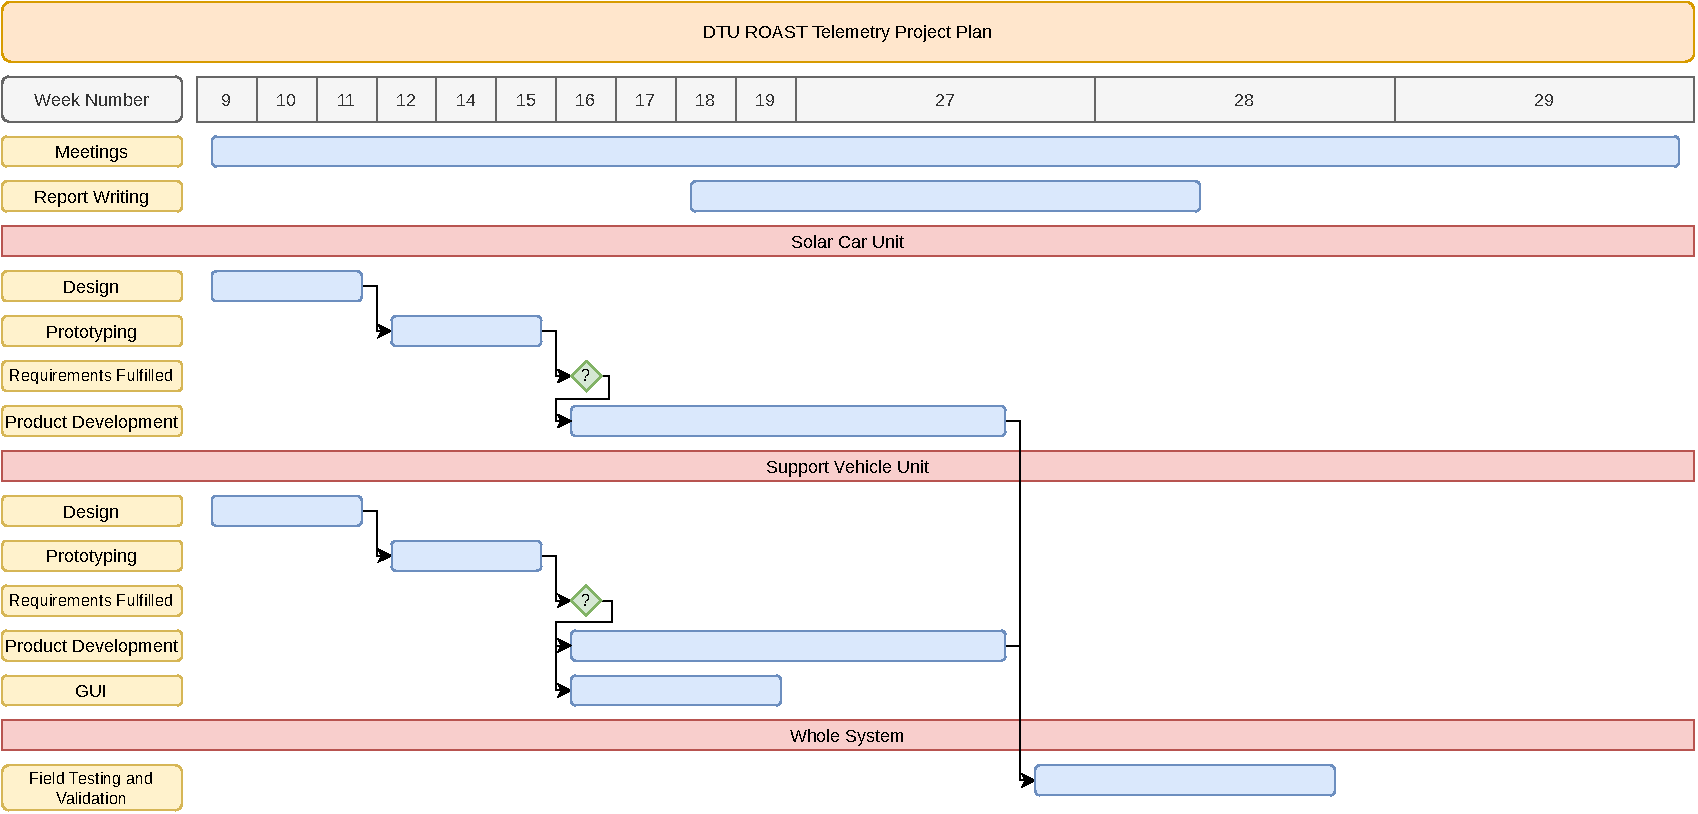
\includegraphics[width=1.45\textwidth]{documentation/images/projectPlan.pdf}
\end{landscape}
\section{Referenceliste}
\begin{thebibliography}{9}
\bibitem{wsc}
Bridgestone World Solar Challenge, 
URL: https://worldsolarchallenge.org/
\end{thebibliography}
\section{Grøn dyst?}
\end{document}